\documentclass{article}

\author{Tran Van Tan Khoi}

\title{Weekly Homework Report \#4}

\date{April 15, 2025}

\usepackage[T1]{fontenc}
\usepackage[utf8]{inputenc}
\usepackage[a4paper,top=2cm,bottom=2cm,left=3cm,right=3cm,marginparwidth=1.75cm]{geometry}
\usepackage[colorlinks=true, allcolors=blue]{hyperref}
\usepackage{graphicx}
\usepackage{listings}

\lstset{language=C++,keywordstyle={\bfseries \color{blue}}}

\begin{document}

\maketitle

\section{About}

Typical implementation of some functions of Singly Linked Lists and Doubly Linked Lists. Access the Github repository via this \href{https://github.com/xtrkoi/throwaway-re}{hyperlink}.

\begin{figure*}[h]
    \centering
    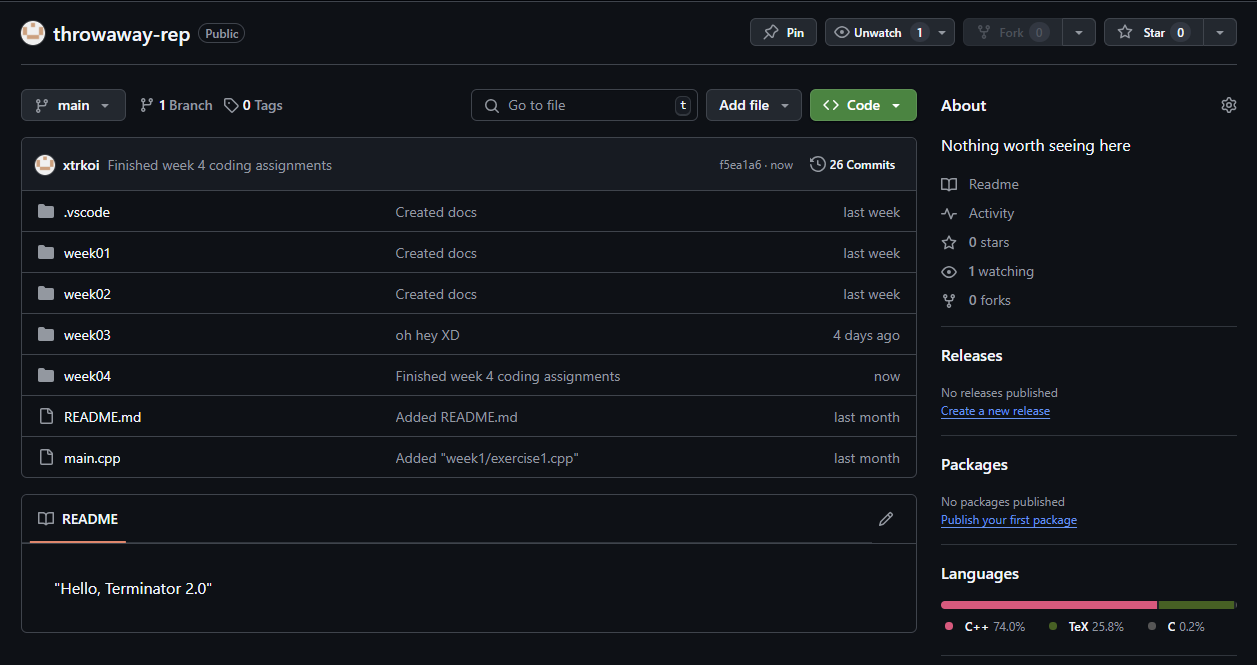
\includegraphics[width=12cm]{images/image.png}
\end{figure*}

\section{Singly Linked List}

Before we begin, there are some auxiliary functions that would help in implementation of the later functions. These include:

\begin{enumerate}
    \item \lstinline{NODE *pred(List *&L, NODE *p_node)}: finds the previous node of \lstinline{p_node} in the list \lstinline{L} (this is especially useful when there is no easy way to access the previous node in singly linked lists).
    \item \lstinline{NODE *succ(List *&L, NODE *p_node)}: finds the next node of \lstinline{p_node} in the list \lstinline{L}.
    \item \lstinline{NODE *find_first_of(List *&L, int key)}: finds the first node in the list \lstinline{L} with given key.
    \item \lstinline{bool remove_node(List *&L, NODE *p_node)}: remove the node with given pointer.
    \item \lstinline{NODE *extract_node(List *&L, int index)}: finds the node with given index.
    \item \lstinline{int extract_index(List L, NODE p_node)}: finds the index of given node.
\end{enumerate}

\subsection{Create a new node}

Creating a new node and returning a pointer to the created node is easily accomplished with the \lstinline{new} operator. Note that if the allocation fails then \lstinline{new} simply returns \lstinline{nullptr}, which is also what we would return in this case. Checking for allocation failure should be done outside this function.

\subsection{Create a new list with a given node}

The \lstinline{List} class already come with a constructor, simply call \lstinline{List(p_node, p_node)} (\lstinline{p_node} is an input parameter).

\subsection{Insert a node with a given key at the front}

Consider two cases: when the list is empty, and when it is not.


When the list is empty, simply attach the \lstinline{p_head} and \lstinline{p_tail} pointer to the newly created node with given key.


When the list isn't empty, make sure the \lstinline{p_next} pointer of the newly created node points the current \lstinline{p_head}. Then modify the \lstinline{p_head} pointer so it points to the node.


\subsection{Insert a node with a given key to the back}

A similar approach can be done by considering two cases of whether the list is empty or not.


When the list is empty, simply attach the \lstinline{p_head} and \lstinline{p_tail} pointer to the newly created node with given key.


When the list isn't empty, change the \lstinline{p_tail}'s \lstinline{p_next} pointer then change the \lstinline{p_tail} pointer itself.


\subsection{Remove the first node}

We can follow every steps in the front-insertion method in a reverse fashion. We only further need to take into account of the the case where the list is already empty.


\subsection{Remove the last node}

Same thing, just the opposite.


\subsection{Remove all nodes without destroying the list}

We assume that we don't deallocate the list itself, only remove all content of the list. There isn't a more straightforward way than removing each node one-by-one.


\subsection{Remove the previous node of the node with given key}

First, find the node with the given key. Then, remove the node before it. This can be all done with auxiliary functions we implemented beforehand.


\subsection{Remove the next node of the node with given key}

We do the same thing as before, but removing the node after instead.


\subsection{Add a node at a given position}

This is where the \lstinline{extract_node} comes in handy. Insertion can be handled by determining the nodes before and after the node to be inserted, with special case can be handled by \lstinline{addHead} and \lstinline{addTail} functions.


\subsection{Remove a node at a given position}

It is much simpler than adding because we can use the \lstinline{extract_node} and \lstinline{remove_node} auxiliary functions.


\subsection{Add a node before the node with given key}

We find the node with the given key then use the function which will add the node at the given position.


\subsection{Add a node after the node with given key}

Almost the same thing, just slightly different.


\subsection{Print all nodes in a list}

Traverse the nodes in the list one at a time and print the key of each node, assuming the list doesn't have loops.


\subsection{Count the number of nodes in a list}

We can traverse the list and increase the count when visiting each node, or find the index of the last node with \lstinline{extract_index} auxiliary function.


\subsection{Reverse a list by creating a new list}

Unlike reversing a linked list in-place, in which we manage some moving pointers, creating a new list which is the reverse of the given list can be easier. Traverse the list from front to back and insert each node to the head of the new list.


\subsection{Remove all duplicate nodes so each node in the list is unique}

An inefficient solution is to traverse the list and remove each node with same key as the current node which isn't the current node itself.


\subsection{Remove all nodes with a given key}

An inefficient solution is to repeatedly find a node with the given key and remove it from the list.



\section{Doubly Linked List}

In a doubly linked list, each node now also has a pointer points to the node preceeding it. This makes insertions and removals a bit more complicated but allows for much faster backward traversal in the list.


\end{document}